\documentclass[10pt,letterpaper]{article}

\usepackage[margin=0.7in]{geometry}
\usepackage{parskip}
\usepackage{enumitem}
\usepackage{xcolor}
\usepackage{titlesec}
\usepackage{fancyhdr}
\usepackage{microtype}
\usepackage{tikz}
\usepackage{float}
\usepackage{tabularx}
\usepackage{array}
\usepackage{booktabs}
\usetikzlibrary{shapes.geometric, arrows.meta, positioning, fit, backgrounds, calc}

\setlength{\parskip}{4pt}
\setlist[itemize]{leftmargin=1.1em,topsep=1pt,itemsep=1pt,parsep=0pt}
\setlist[enumerate]{leftmargin=1.3em,topsep=1pt,itemsep=1pt,parsep=0pt}

\titleformat{\section}{\large\bfseries}{}{0pt}{}
\titlespacing*{\section}{0pt}{8pt}{2pt}
\titleformat{\subsection}{\normalsize\bfseries}{}{0pt}{}
\titlespacing*{\subsection}{0pt}{4pt}{1pt}

\pagestyle{fancy}
\fancyhf{}
\rhead{\small Microbiology LIMS POC --- v3.2 (visual)}
\lhead{\small Process Reference + Block Diagrams}
\rfoot{\small \thepage}

% palette mirrors the drawio
\definecolor{srcfill}{HTML}{DAE8FC}
\definecolor{srcdraw}{HTML}{6C8EBF}
\definecolor{cmpfill}{HTML}{F5F5F5}
\definecolor{cmpdraw}{HTML}{666666}
\definecolor{aifill}{HTML}{E1D5E7}
\definecolor{aidraw}{HTML}{9673A6}
\definecolor{outfill}{HTML}{D5E8D4}
\definecolor{outdraw}{HTML}{82B366}
\definecolor{valfill}{HTML}{FFF2CC}
\definecolor{valdraw}{HTML}{D6B656}
\definecolor{xfill}{HTML}{FFE6CC}
\definecolor{xdraw}{HTML}{D79B00}
\definecolor{notefill}{HTML}{FAFAFA}
\definecolor{tablehd}{HTML}{F0F0F0}

\tikzset{
  blk/.style={rectangle, rounded corners=2pt, line width=0.5pt, align=center, font=\scriptsize, inner sep=3pt, minimum height=0.85cm},
  src/.style={blk, draw=srcdraw, fill=srcfill, minimum width=1.95cm},
  cmp/.style={blk, draw=cmpdraw, fill=cmpfill, minimum width=1.95cm},
  ai/.style={blk, draw=aidraw, fill=aifill, minimum width=1.95cm},
  dst/.style={blk, draw=outdraw, fill=outfill, minimum width=1.95cm},
  val/.style={blk, draw=valdraw, fill=valfill, minimum width=1.95cm},
  xcut/.style={blk, draw=xdraw, fill=xfill, minimum width=1.95cm},
  decision/.style={diamond, aspect=2.2, draw=valdraw, fill=valfill, line width=0.5pt, align=center, font=\scriptsize, inner sep=1pt},
  io/.style={rectangle, draw=cmpdraw, dashed, fill=notefill, align=left, font=\tiny\ttfamily, line width=0.3pt, inner sep=3pt},
  lab/.style={font=\tiny\itshape, text=black!60},
  arr/.style={->, >={Stealth[length=4pt]}, line width=0.5pt, draw=black!70},
  arrdash/.style={->, >={Stealth[length=4pt]}, line width=0.5pt, draw=xdraw, dashed},
}

\renewcommand{\arraystretch}{1.15}

\begin{document}

\begin{center}
{\Large\bfseries Microbiology LIMS POC --- Process Reference (with Block Diagrams)}\\[2pt]
{\small v3.2 (Conditioned Discovery) \quad\textbar\quad Visual companion to \texttt{microbio\_lims\_architecture.drawio} \quad\textbar\quad 2026-04-29}
\end{center}

\section{What the system does}

A subject-matter expert (SME) drops microbiology SOPs into S3. An agent pipeline, grounded in a hybrid retrieval substrate (BM25 + dense), reads them and emits two artifacts: \textbf{(A)} a Jira-ready Epic / Story tree, and \textbf{(B)} per-culture YAML configuration profiles (urine, blood, target-pathogen).

The Cytology Jira backlog is used as a \emph{teaching corpus} (few-shot exemplars), not a registry to match against. The agent stops at Story --- Tasks (test IDs, library versions, DB columns) are dev-authored once the team has codebase visibility.

\textbf{v3.2 addition --- Conditioned Discovery.} v3.1 generated epics from-scratch and treated themes G1--G8 as a closed Cyto-derived vocabulary. v3.2 adds a \emph{warm-start} step at both levels: a new pre-flight \textbf{Theme Discovery agent} bootstraps a discipline's theme catalog by classifying its SOPs against the prior taxonomy first and surfacing only the residual as novel; the \textbf{Epic Extractor runs in conditioned mode}, classifying drafts against the prior epic catalog (\texttt{cyto\_epic\_v1}) before clustering anything new. The result: most themes and epics inherit by construction with explicit lineage, and only genuinely-novel structure (with cluster evidence) goes to SME for ratification. See the v3.2 sections below.

\textbf{Color legend:} \tikz[baseline=-0.5ex]\node[src,minimum width=0.7cm,minimum height=0.4cm,inner sep=1pt,font=\tiny]{src};\, source/data \quad
\tikz[baseline=-0.5ex]\node[cmp,minimum width=0.7cm,minimum height=0.4cm,inner sep=1pt,font=\tiny]{cmp};\, compute \quad
\tikz[baseline=-0.5ex]\node[ai,minimum width=0.7cm,minimum height=0.4cm,inner sep=1pt,font=\tiny]{ai};\, AI/LLM agent \quad
\tikz[baseline=-0.5ex]\node[val,minimum width=0.7cm,minimum height=0.4cm,inner sep=1pt,font=\tiny]{val};\, validator/decision \quad
\tikz[baseline=-0.5ex]\node[dst,minimum width=0.7cm,minimum height=0.4cm,inner sep=1pt,font=\tiny]{store};\, storage/output \quad
\tikz[baseline=-0.5ex]\node[xcut,minimum width=0.7cm,minimum height=0.4cm,inner sep=1pt,font=\tiny]{xc};\, cross-cutting

% =====================================================================
\section{Key terms (glossary)}
% =====================================================================

\begin{tabularx}{\textwidth}{@{}>{\bfseries}p{2.5cm}X@{}}
\toprule
SOP & Standard Operating Procedure --- the source document the agent reads.\\
Epic & A capability domain; maps to a Jira Epic. E.g.\ \emph{Microbiology Specimen Receipt}.\\
Story & A dev-actionable unit emitted by the agent. Each Story declares one of four \texttt{shape} values. Maps to a Jira Story.\\
Shape & Categorization assigned to each Story at extraction time. Drives Validator routing and downstream interpretation. Four values: \texttt{capability}, \texttt{workflow-stage-split}, \texttt{configuration-instance}, \texttt{cleanup}.\\
Theme (G1--G8) & Eight content tags spanning the LIMS workflow: G1 Pre-Analytic, G2 Analytic, G3 Post-Analytic, G4 Reporting, G5 QC, G6 Compliance, G7 Instrumentation, G8 Platform. Multi-label per chunk.\\
Teaching corpus & Curated SME-validated (SOP excerpt $\rightarrow$ Story) pairs from Cyto. Used as few-shot exemplars at extraction time.\\
Retrieval slot & A parallel retrieval channel scoped to a particular discipline + theme combination. Up to 5 slots fire per query.\\
Intent & Structured interpretation of a user query: \texttt{\{action, themes, discipline, granularity, refs, confidence\}}.\\
$\tau$ (tau) & Intent-confidence threshold ($0.7$). Below this, the system asks a clarifying question rather than retrieving.\\
$\theta$ (theta) & Retrieval-relevance threshold ($0.5$). If every slot falls below this, the system refuses to generate.\\
Batch wait & The pipeline pause between Validator gate \#1 and Cross-SOP Synthesis. Synthesis cannot run until every per-SOP Story has cleared gate \#1.\\
\midrule
\multicolumn{2}{@{}l}{\itshape v3.2 additions:}\\
Conditioned discovery & A four-pass procedure (classify $\rightarrow$ cluster residual $\rightarrow$ SME ratify $\rightarrow$ re-tag) that warm-starts a new catalog against an existing prior, rather than clustering from scratch. Applied at both theme and epic levels.\\
Prior catalog & The existing themes (or epics) that conditioned discovery treats as the structure-to-reuse. Cyto's catalogs are the prior for both Micro and Histology bootstraps.\\
Residual & Inputs whose classification confidence falls below $\tau_{\text{match}}$ in Pass 1. Only residuals are clustered for novelty.\\
$\tau_{\text{match}}$ & Match-confidence threshold for Pass 1 (default $0.65$). Distinct from the query-time $\tau$ above. Higher $\tau_{\text{match}}$ $\Rightarrow$ eager-to-inherit.\\
$\varepsilon_{\text{novelty}}$ & Minimum cluster size in Pass 2 (default $3$). Higher $\Rightarrow$ stricter evidence bar before admitting a novel theme/epic.\\
G0 / E0 & First-class \emph{unclassified} bucket on every theme catalog (G0) and epic catalog (E0). 5\% alarm threshold over a rolling window triggers re-running discovery.\\
Catalog versioning & Theme catalogs are named \texttt{<discipline>\_v<N>} (e.g.\ \texttt{cyto\_v1}, \texttt{histo\_v1}); epic catalogs are named \texttt{<discipline>\_epic\_v<N>} (e.g.\ \texttt{cyto\_epic\_v1}). They version independently. Stories carry a \texttt{theme\_catalog\_version} field for theme resolution.\\
ANALOGY map & Explicit cross-catalog link table. Each link typed: \texttt{identical} / \texttt{partial} / \texttt{discarded\_in\_target} / \texttt{novel\_in\_target}. Replaces v3.1's implicit shared-theme assumption.\\
\bottomrule
\end{tabularx}

% =====================================================================
\section{Agent pipeline --- 5 agents, Validator gates twice}
% =====================================================================

\begin{figure}[H]
\centering
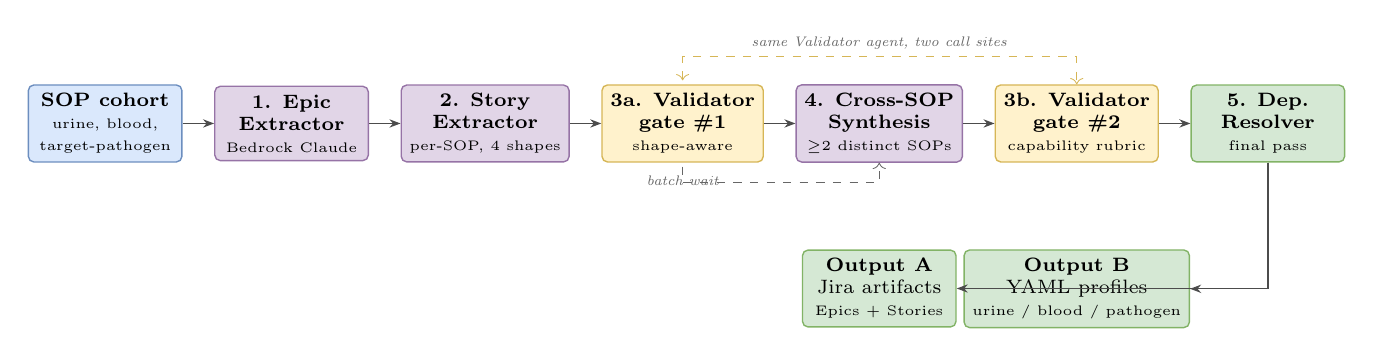
\begin{tikzpicture}[node distance=0.35cm and 0.4cm]
  \node[src] (sop) {\textbf{SOP cohort}\\\tiny urine, blood,\\\tiny target-pathogen};
  \node[ai, right=of sop] (epic) {\textbf{1. Epic}\\\textbf{Extractor}\\\tiny Bedrock Claude};
  \node[ai, right=of epic] (story) {\textbf{2. Story}\\\textbf{Extractor}\\\tiny per-SOP, 4 shapes};
  \node[val, right=of story] (val1) {\textbf{3a. Validator}\\\textbf{gate \#1}\\\tiny shape-aware};
  \node[ai, right=of val1] (synth) {\textbf{4. Cross-SOP}\\\textbf{Synthesis}\\\tiny $\geq$2 distinct SOPs};
  \node[val, right=of synth] (val2) {\textbf{3b. Validator}\\\textbf{gate \#2}\\\tiny capability rubric};
  \node[dst, right=of val2] (deps) {\textbf{5. Dep.}\\\textbf{Resolver}\\\tiny final pass};
  \draw[arr] (sop) -- (epic);
  \draw[arr] (epic) -- (story);
  \draw[arr] (story) -- (val1);
  \draw[arr] (val1) -- (synth);
  \draw[arr] (synth) -- (val2);
  \draw[arr] (val2) -- (deps);
  \node[lab, below=0.05cm of val1] (bw) {batch wait};
  \draw[->, dashed, draw=cmpdraw, line width=0.3pt] (val1.south) ++(0,-0.05) -- ++(0,-0.20) -| (synth.south);
  \node[dst, below=1.1cm of synth] (jira) {\textbf{Output A}\\Jira artifacts\\\tiny Epics + Stories};
  \node[dst, below=1.1cm of val2] (yaml) {\textbf{Output B}\\YAML profiles\\\tiny urine / blood / pathogen};
  \draw[arr] (deps.south) |- (yaml.east);
  \draw[arr] (deps.south) |- (jira.east);
  \draw[<->, dashed, draw=valdraw, line width=0.3pt]
    (val1.north) ++(0,0.05) -- ++(0,0.30) -| (val2.north);
  \node[lab, above=0.32cm of synth] {same Validator agent, two call sites};
\end{tikzpicture}
\end{figure}

\begin{enumerate}
  \item \textbf{Epic Extractor} --- identifies capability domains. \emph{Out:} Epic record per domain.
  \item \textbf{Story Extractor} --- per-SOP, multi-shape. Different elements of one SOP can take different shapes.
  \item \textbf{Validator gate \#1} --- shape verification + shape-specific sub-rubric. Two revisions then SME-escalate.
  \item \textbf{Cross-SOP Synthesis} --- runs after gate \#1 clears the entire batch. Behavioral-similarity clustering over (title + AC + source excerpt); cluster qualifies only if its members come from $\geq 2$ \emph{distinct} SOPs. Lifts a capability Story per cluster, with \texttt{cross\_links[]} back to the contributing concretes.
  \item \textbf{Validator gate \#2} --- same Validator agent as gate \#1, second call site; capability rubric only. Synthesized stories are a \emph{new} artifact, not a derivative, so they re-pass the bar.
  \item \textbf{Dependency Resolver} --- story$\leftrightarrow$story dependencies, stage-split sibling links, capability$\leftrightarrow$child links. Finalizes the artifact graph for Jira push.
\end{enumerate}

\textbf{v3.2 modifications inside the main pipeline:} the Epic Extractor (1) gains \emph{conditioned mode} --- it classifies its drafts against the prior epic catalog before clustering anything as novel. The other four agents are unchanged in shape. A \emph{new sixth agent} --- the \textbf{Theme Discovery agent} --- runs as pre-flight (one-time per discipline), not on the per-SOP critical path. Both are detailed in the next two sections.

% =====================================================================
\section{v3.2 Theme Discovery --- pre-flight, one-time per discipline}
% =====================================================================

Theme Discovery runs \emph{before} the main pipeline boots for a new discipline (and again only when the G0 alarm trips). Its job: emit a versioned theme catalog (e.g.\ \texttt{histo\_v1}) by warm-starting against an existing prior (e.g.\ \texttt{cyto\_v1}). Most themes inherit; novel ones must clear an evidence bar and an SME gate.

\begin{figure}[H]
\centering
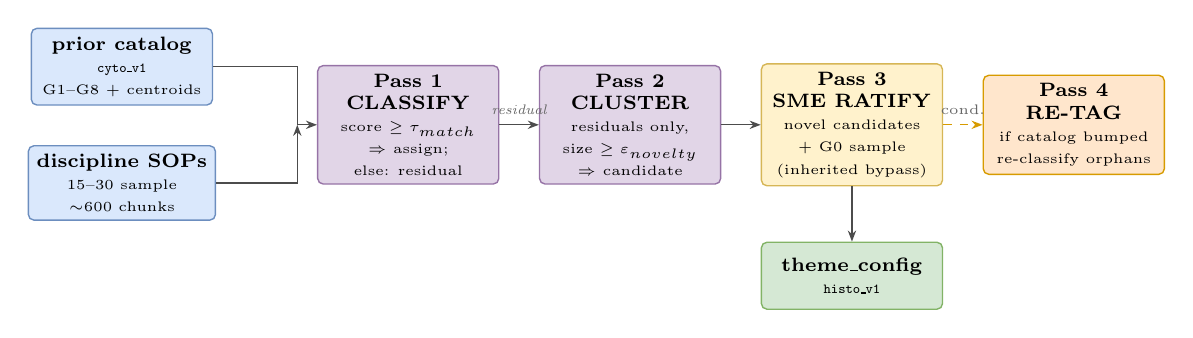
\begin{tikzpicture}[node distance=0.45cm and 0.5cm]
  \node[src, minimum width=2.3cm] (prior) {\textbf{prior catalog}\\\tiny \texttt{cyto\_v1}\\\tiny G1--G8 + centroids};
  \node[src, minimum width=2.3cm, below=0.5cm of prior] (sops) {\textbf{discipline SOPs}\\\tiny \mbox{15--30 sample}\\\tiny $\sim$600 chunks};
  \coordinate (mid) at ($(prior.east)!0.5!(sops.east)$);
  \node[ai, minimum width=2.3cm, right=1.3cm of mid] (p1) {\textbf{Pass 1}\\\textbf{CLASSIFY}\\\tiny score $\geq \tau_{\text{match}}$\\\tiny $\Rightarrow$ assign;\\\tiny else: residual};
  \node[ai, minimum width=2.3cm, right=of p1] (p2) {\textbf{Pass 2}\\\textbf{CLUSTER}\\\tiny residuals only,\\\tiny size $\geq \varepsilon_{\text{novelty}}$\\\tiny $\Rightarrow$ candidate};
  \node[val, minimum width=2.3cm, right=of p2] (p3) {\textbf{Pass 3}\\\textbf{SME RATIFY}\\\tiny novel candidates\\\tiny + G0 sample\\\tiny (inherited bypass)};
  \node[xcut, minimum width=2.3cm, right=of p3] (p4) {\textbf{Pass 4}\\\textbf{RE-TAG}\\\tiny if catalog bumped\\\tiny re-classify orphans};
  \node[dst, minimum width=2.3cm, below=0.7cm of p3] (cfg) {\textbf{theme\_config}\\\tiny \texttt{histo\_v1}};
  \draw[arr] (prior) -| ($(p1.west)+(-0.25,0)$) -- (p1.west);
  \draw[arr] (sops) -| ($(p1.west)+(-0.25,0)$);
  \draw[arr] (p1) -- node[lab, above]{residual} (p2);
  \draw[arr] (p2) -- (p3);
  \draw[arrdash] (p3) -- node[lab, above, font=\tiny]{cond.} (p4);
  \draw[arr] (p3) -- (cfg);
\end{tikzpicture}
\caption{Theme Discovery --- four passes, pre-flight per discipline. Pass 4 fires only when SME ratification changes the catalog (novel ratified or theme discarded).}
\end{figure}

\textbf{Algorithm in pseudocode:}

\noindent\texttt{\scriptsize PASS 1 (CLASSIFY): for each chunk: score = best\_match(chunk, prior); if score $\geq\tau_{\text{match}}$ assign else residual\\
PASS 2 (CLUSTER): cluster residuals (HDBSCAN); each cluster of size $\geq\varepsilon_{\text{novelty}}$ $\rightarrow$ candidate\_novel\_theme\\
PASS 3 (SME GATE): SME confirms / renames / rejects each novel candidate; inherited themes pass automatically\\
PASS 4 (RE-TAG, if catalog changed): re-classify previously-tagged corpus chunks against catalog\_v(N+1)}

\textbf{Two knobs control the bias.} $\tau_{\text{match}}$ (default $0.65$): higher $\Rightarrow$ eager-to-inherit (small residual; risk forced fits). $\varepsilon_{\text{novelty}}$ (default $3$): higher $\Rightarrow$ stricter evidence bar before admitting novelty. The user's stated motive --- ``don't just end up with entirely new ones'' --- corresponds to a high $\tau_{\text{match}}$ and a non-trivial $\varepsilon_{\text{novelty}}$.

\textbf{Worked example --- bootstrapping Histology from \texttt{cyto\_v1}.} Pass 1 classifies $460/600$ chunks into G1--G8 (residual $= 140$, including 12 chunks that fit G7 above $\tau_{\text{match}}$). Pass 2 finds 4 clusters above $\varepsilon_{\text{novelty}}$: H1 Tissue Processing (38), H2 Staining (32), H3 Block Archive (25), H4 Frozen Section (23); 22 chunks $\rightarrow$ G0 (3.7\%, below alarm). Pass 3: SME confirms all 4 novel themes; flags G7 as redundant in histo (instrument concerns fold into H1) --- discarded. Pass 4 re-classifies the 12 G7-orphaned chunks against the post-discard taxonomy (most land in H1, consistent with the ANALOGY map's \texttt{G7$\rightarrow$H1, partial} link). Final \texttt{histo\_v1}: 11 active themes (7 inherited + 4 novel; G7 recorded in ANALOGY map only). Reuse rate: 7/11 $\approx$ 64\%; 7/8 of the prior themes (87.5\%) survived.

% =====================================================================
\section{v3.2 Conditioned Epic Extractor --- match before generate}
% =====================================================================

In v3.1 the Epic Extractor proposed Micro epics from-scratch and optionally annotated \texttt{cyto\_epic\_analog} post-hoc when retrieval signal happened to align. In v3.2 the order is reversed: drafts are classified against the prior epic catalog \emph{first}; matched drafts inherit the analog by construction; only residuals get clustered for novelty.

\begin{figure}[H]
\centering
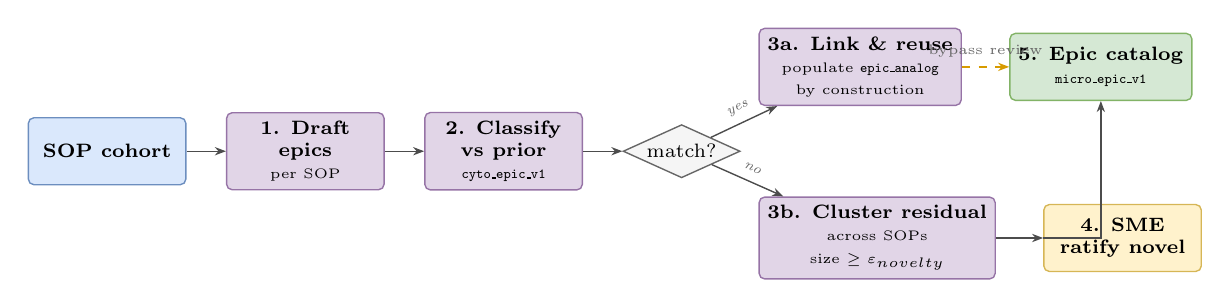
\begin{tikzpicture}[node distance=0.4cm and 0.5cm]
  \node[src, minimum width=2.0cm] (sops) {\textbf{SOP cohort}};
  \node[ai, minimum width=2.0cm, right=of sops] (drafts) {\textbf{1. Draft}\\\textbf{epics}\\\tiny per SOP};
  \node[ai, minimum width=2.0cm, right=of drafts] (cls) {\textbf{2. Classify}\\\textbf{vs prior}\\\tiny \texttt{cyto\_epic\_v1}};
  \node[decision, fill=cmpfill, draw=cmpdraw, right=of cls] (dec) {match?};
  \node[ai, minimum width=2.4cm, above right=0.4cm and 0.6cm of dec] (link) {\textbf{3a. Link \& reuse}\\\tiny populate \texttt{epic\_analog}\\\tiny by construction};
  \node[ai, minimum width=2.4cm, below right=0.4cm and 0.6cm of dec] (clust) {\textbf{3b. Cluster residual}\\\tiny across SOPs\\\tiny size $\geq \varepsilon_{\text{novelty}}$};
  \node[val, minimum width=2.0cm, right=0.6cm of clust] (sme) {\textbf{4. SME}\\\textbf{ratify novel}};
  \node[dst, minimum width=2.3cm, right=0.6cm of link] (cat) {\textbf{5. Epic catalog}\\\tiny \texttt{micro\_epic\_v1}};
  \draw[arr] (sops) -- (drafts);
  \draw[arr] (drafts) -- (cls);
  \draw[arr] (cls) -- (dec);
  \draw[arr] (dec) -- node[lab, sloped, above]{yes} (link);
  \draw[arr] (dec) -- node[lab, sloped, above]{no} (clust);
  \draw[arr] (clust) -- (sme);
  \draw[arrdash] (link) -- node[lab, above, font=\tiny]{bypass review} (cat);
  \draw[arr] (sme) -| (cat);
\end{tikzpicture}
\caption{Conditioned Epic Extractor --- the ``match?'' decision is algorithmic (not SME-gated; hence neutral coloring). Only the novel branch goes through SME ratification.}
\end{figure}

\textbf{Result for the Micro POC:} most Micro epics inherit Cyto's structure with explicit \texttt{epic\_analog} populated by construction; only genuinely novel epics --- e.g.\ Antibiotic Susceptibility Testing (AST), if it has no Cyto analog --- emerge with cluster evidence. The dev team reads \texttt{micro\_epic\_v1} and immediately sees what's reused vs.\ new without having to do the mapping themselves.



A \textbf{shape} is the categorization the Story Extractor assigns to each Story. It tells the Validator which sub-rubric to apply, and tells downstream consumers (devs, the YAML emitter) how to interpret the AC. Per-SOP extraction picks one of four shapes per element. Cross-SOP synthesis only ever emits the \texttt{capability} shape.

\begin{tabularx}{\textwidth}{@{}>{\ttfamily}p{3.2cm}p{6.5cm}X@{}}
\toprule
\textbf{shape} & \textbf{Use when\ldots} & \textbf{Validator rubric} \\
\midrule
capability & SOP describes a configurable system feature you can imagine multiple labs/cultures parameterizing & MUST/SHALL on AC; testable; configurability boundaries explicit \\
workflow-stage-split & Same capability, but SOP describes different behavior at different workflow stages (before / during / after results) & Stage explicit in title; sibling stories enumerated and cross-linked \\
configuration-instance & Concrete data values for one culture / lab. \emph{No new feature --- just data.} & Typed values + verbatim citation. \emph{No MUST/SHALL.} \\
cleanup & Modify or remove an existing artifact. \emph{No new feature.} & Target named + before/after observable + regression risk \\
\bottomrule
\end{tabularx}

\begin{figure}[H]
\centering
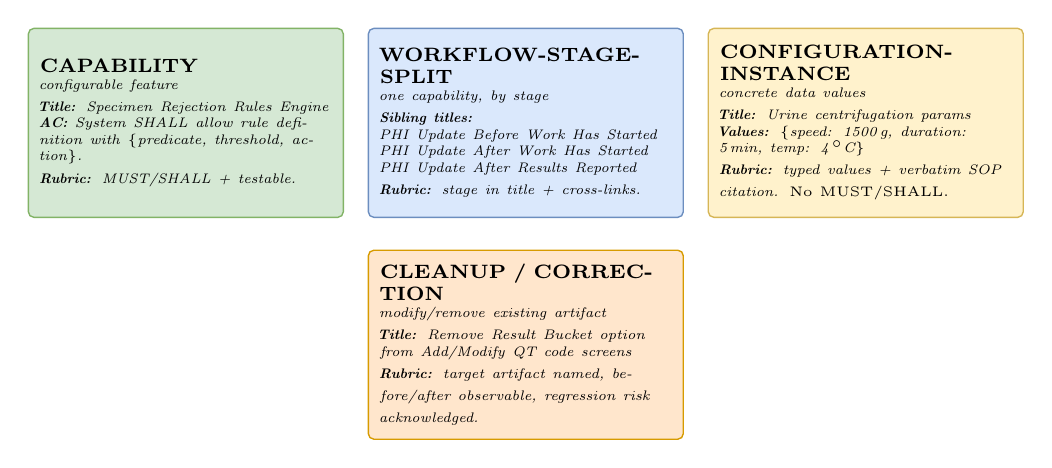
\begin{tikzpicture}[node distance=0.3cm]
  \node[blk, draw=outdraw, fill=outfill, minimum width=4.0cm, minimum height=2.4cm, align=left, text width=3.7cm] (s1)
    {\textbf{CAPABILITY}\\\tiny\itshape configurable feature\\[2pt]
     \tiny\textbf{Title:} Specimen Rejection Rules Engine\\
     \tiny\textbf{AC:} System SHALL allow rule definition with \{predicate, threshold, action\}.\\
     \tiny\textbf{Rubric:} MUST/SHALL + testable.};
  \node[blk, draw=srcdraw, fill=srcfill, right=of s1, minimum width=4.0cm, minimum height=2.4cm, align=left, text width=3.7cm] (s2)
    {\textbf{WORKFLOW-STAGE-SPLIT}\\\tiny\itshape one capability, by stage\\[2pt]
     \tiny\textbf{Sibling titles:}\\
     \tiny PHI Update Before Work Has Started\\
     \tiny PHI Update After Work Has Started\\
     \tiny PHI Update After Results Reported\\
     \tiny\textbf{Rubric:} stage in title + cross-links.};
  \node[blk, draw=valdraw, fill=valfill, right=of s2, minimum width=4.0cm, minimum height=2.4cm, align=left, text width=3.7cm] (s3)
    {\textbf{CONFIGURATION-INSTANCE}\\\tiny\itshape concrete data values\\[2pt]
     \tiny\textbf{Title:} Urine centrifugation params\\
     \tiny\textbf{Values:} \{speed: 1500\,g, duration: 5\,min, temp: 4\,$^\circ$C\}\\
     \tiny\textbf{Rubric:} typed values + verbatim SOP citation. \emph{No MUST/SHALL.}};
  \node[blk, draw=xdraw, fill=xfill, below=0.4cm of s2, minimum width=4.0cm, minimum height=2.4cm, align=left, text width=3.7cm] (s4)
    {\textbf{CLEANUP / CORRECTION}\\\tiny\itshape modify/remove existing artifact\\[2pt]
     \tiny\textbf{Title:} Remove Result Bucket option from Add/Modify QT code screens\\
     \tiny\textbf{Rubric:} target artifact named, before/after observable, regression risk acknowledged.};
\end{tikzpicture}
\end{figure}

% =====================================================================
\section{Schemas --- deep dive}
% =====================================================================

\textbf{Note on IDs:} draft IDs (e.g.\ \texttt{epic\_draft\_3}, \texttt{story\_draft\_42}) are used in-pipeline; the Dependency Resolver replaces them with final Jira-shaped IDs (e.g.\ \texttt{EPIC-MICRO-001}, \texttt{STORY-MICRO-1042}) at Jira-push time.

\subsection{Epic schema (v3.2)}

\noindent\texttt{\scriptsize \{ id: "EPIC-MICRO-001", title: "Microbiology Specimen Receipt",\\
\hspace*{1em}description: "...", discipline: "microbiology",\\
\hspace*{1em}themes: ["G1","G5"], theme\_catalog\_version: "cyto\_v1",\\
\hspace*{1em}epic\_analog: \{ catalog\_id: "cyto\_epic\_v1", epic\_id: "EPIC-CYTO-007", equivalence: "identical" \},\\
\hspace*{1em}inheritance\_basis: \{ match\_score: 0.78, shared\_themes: ["G1"], auto\_inherited: true \} \}}

\begin{tabularx}{\textwidth}{@{}>{\ttfamily}p{3.2cm}p{2.0cm}p{1.4cm}X@{}}
\toprule
\textbf{field} & \textbf{type} & \textbf{req'd} & \textbf{notes} \\
\midrule
id & string & yes & Jira-shaped Epic ID. \\
title & string & yes & Short capability-domain name. \\
description & string & yes & 1--3 sentence scope statement. \\
discipline & enum & yes & \texttt{microbiology} $|$ \texttt{histology} $|$ \texttt{cytology}. \\
themes[] & array & yes & Multi-label tags; values drawn from the theme catalog named by \texttt{theme\_catalog\_version}. \\
theme\_catalog\_version & string & yes & \emph{(v3.2)} The theme catalog these tags resolve in --- e.g.\ \texttt{cyto\_v1} for Micro POC, \texttt{histo\_v1} for Histology. \\
epic\_analog & object & no & \emph{(v3.2 --- replaces \texttt{cyto\_epic\_analog})} Cross-catalog link: \texttt{\{catalog\_id, epic\_id, equivalence\}}. Populated by the conditioned Epic Extractor when \texttt{match\_score $\geq \tau_{\text{match}}$}. \\
inheritance\_basis & object & no & \emph{(v3.2)} Provenance for inherited epics: \texttt{\{match\_score, shared\_themes[], auto\_inherited\}}. Absent for novel epics; those carry \texttt{novelty\_basis} instead. \\
\bottomrule
\end{tabularx}

\subsection{Story schema}

\noindent\texttt{\scriptsize \{ id: "STORY-MICRO-1042", epic\_id: "EPIC-MICRO-001", shape: "capability",\\
\hspace*{1em}title: "Configurable specimen rejection rules engine", description: "...",\\
\hspace*{1em}acceptance\_criteria: [\{when, then, expected\_value?\}, ...],\\
\hspace*{1em}source\_citations: [\{doc\_id, section, line\_range\}, ...],\\
\hspace*{1em}dependencies: ["STORY-MICRO-1018"],\\
\hspace*{1em}cross\_links:  ["STORY-MICRO-1043","STORY-MICRO-1044","STORY-MICRO-1045"],\\
\hspace*{1em}estimated\_complexity: "M", edge\_cases\_handled: [...],\\
\hspace*{1em}status: "validated", source\_chunks: ["chunk\_001","chunk\_017"] \}}

\begin{tabularx}{\textwidth}{@{}>{\ttfamily}p{3.4cm}p{3.0cm}p{1.2cm}X@{}}
\toprule
\textbf{field} & \textbf{type} & \textbf{req'd} & \textbf{notes} \\
\midrule
id & string & yes & Jira-shaped Story ID. \\
epic\_id & string & yes & FK to parent Epic. \\
shape & enum (4) & yes & Drives Validator routing. \\
title & string & yes & Concrete + unambiguous; for stage-split, must name the stage. \\
description & string & yes & User-story format for capability/stage-split; descriptive prose for config-instance/cleanup. \\
acceptance\_criteria[] & array & yes & Capability/stage-split: MUST/SHALL phrasing. Config-instance: \texttt{expected\_value} populated. Cleanup: before/after wording. \\
source\_citations[] & array $\langle$\{doc\_id, section, line\_range\}$\rangle$ & yes & Must resolve to indexed chunks; verbatim excerpt for config-instance. \\
dependencies[] & array $\langle$Story ID$\rangle$ & no & Stories that must complete before this one is workable. \\
cross\_links[] & array $\langle$Story ID$\rangle$ & no & Capability $\leftrightarrow$ concrete contributors; stage-split sibling group. Backbone of the Story DAG. \\
technical\_hints & string & no & Dev-facing guidance. \\
estimated\_complexity & enum \texttt{S}$|$\texttt{M}$|$\texttt{L} & yes & Heuristic, sprint sizing. \\
edge\_cases\_handled[] & array of strings & no & Surfaced corner cases. \\
status & enum & yes & \texttt{draft} $|$ \texttt{validated} $|$ \texttt{ready}. \\
source\_chunks[] & array $\langle$chunk ID$\rangle$ & yes & Audit trail to the retrieval substrate. \\
\bottomrule
\end{tabularx}

\subsection{Cluster schema (intermediate, in Cross-SOP Synthesis)}

Not persisted to Jira; lives only between gate \#1 and gate \#2 in memory.

\noindent\texttt{\scriptsize \{ cluster\_id: "clust\_rejection\_3sop",\\
\hspace*{1em}member\_story\_ids: ["STORY-MICRO-1043","STORY-MICRO-1044","STORY-MICRO-1045"],\\
\hspace*{1em}source\_sops: ["doc\_micro\_014\_v3","doc\_micro\_022\_v1","doc\_micro\_037\_v2"],\\
\hspace*{1em}centroid\_summary: "Reject specimen on a culture-specific predicate.",\\
\hspace*{1em}proposed\_capability\_title: "Configurable specimen rejection rules engine" \}}

A cluster qualifies for lifting \textbf{iff} \texttt{len(unique(source\_sops)) >= 2}. Two stories from the same SOP do not qualify, even if they cluster tightly.

\subsection{Validator output schema}

\noindent\texttt{\scriptsize \{ story\_id: "STORY-MICRO-1042", verdict: "revise",\\
\hspace*{1em}shape\_declared: "capability", shape\_verified: "capability",\\
\hspace*{1em}failed\_checks: [\\
\hspace*{2em}\{rule:"must\_shall\_present", severity:"error", message:"AC 1 lacks MUST/SHALL phrasing."\},\\
\hspace*{2em}\{rule:"ambiguous\_quantifier", severity:"error", message:"AC 2 uses 'appropriate'."\}\\
\hspace*{1em}], attempt: 1 \}}

\begin{tabularx}{\textwidth}{@{}>{\ttfamily}p{2.6cm}p{3.0cm}X@{}}
\toprule
\textbf{field} & \textbf{type} & \textbf{notes} \\
\midrule
story\_id & string & The Story under review.\\
verdict & enum & \texttt{accept} (passes), \texttt{revise} (return to extractor with \texttt{failed\_checks}, attempt $<$ 2), or \texttt{escalate} (after 2 failed revisions; SME-routed).\\
shape\_declared & enum & The shape the Story Extractor assigned.\\
shape\_verified & enum & The shape the Validator believes is correct. If it differs from \texttt{shape\_declared}, verdict is automatically \texttt{revise}.\\
failed\_checks[] & array $\langle$\{rule, severity, message\}$\rangle$ & Empty when \texttt{verdict = accept}.\\
attempt & integer & 1 or 2 (after 2, verdict becomes \texttt{escalate}).\\
\bottomrule
\end{tabularx}

\subsection{Theme catalog schema (v3.2)}

\noindent\texttt{\scriptsize catalog\_id: histo\_v1\\
parent\_catalog: cyto\_v1\\
discipline: histology\\
inherited\_themes:\\
\hspace*{1em}- \{ id: G1, name: Pre-Analytic, source: cyto\_v1, match\_count: 142 \}\\
\hspace*{1em}\ldots\\
novel\_themes:\\
\hspace*{1em}- \{ id: H1, name: Tissue Processing, source: histo\_v1,\\
\hspace*{2em}cluster\_evidence: \{n\_chunks: 38, sample\_excerpts: [\ldots]\}, sme\_confirmed: true \}\\
discarded\_themes:\\
\hspace*{1em}- \{ id: G7, reason: "Folded into H1 (partial)", chunks\_re\_tagged: 12 \}\\
unclassified\_bucket: \{ count: 22, pct\_of\_total: 3.7 \}}

\begin{tabularx}{\textwidth}{@{}>{\ttfamily}p{3.4cm}p{1.8cm}p{1.4cm}X@{}}
\toprule
\textbf{field} & \textbf{type} & \textbf{req'd} & \textbf{notes} \\
\midrule
catalog\_id & string & yes & \texttt{<discipline>\_v<N>}. Stories reference this in \texttt{theme\_catalog\_version}. \\
parent\_catalog & string\,$|$\,null & yes & The prior the discovery was conditioned on. \texttt{null} only for the very first ever (\texttt{cyto\_v1}). \\
inherited\_themes[] & array & yes & Themes that survived from \texttt{parent\_catalog} after Pass 1. Each has \texttt{source: <parent>} and a \texttt{match\_count}. \\
novel\_themes[] & array & yes & SME-ratified novelties from Pass 2. Each carries \texttt{cluster\_evidence}. May be empty. \\
discarded\_themes[] & array & opt & Parent themes the SME dropped. \texttt{chunks\_re\_tagged} records the Pass 4 fixup count. \\
unclassified\_bucket & object & yes & G0 stats: \texttt{\{count, pct\_of\_total, sample\_excerpts, next\_review\_due\}}. Always present. 5\% alarm threshold. \\
\bottomrule
\end{tabularx}

\subsection{Epic catalog schema (v3.2)}

\noindent\texttt{\scriptsize catalog\_id: micro\_epic\_v1\\
parent\_catalog: cyto\_epic\_v1\\
discipline: microbiology\\
inherited\_epics:\\
\hspace*{1em}- \{ id: EPIC-MICRO-001, title: Specimen Receiving,\\
\hspace*{2em}epic\_analog: \{catalog\_id: cyto\_epic\_v1, epic\_id: EPIC-CYTO-014, equivalence: identical\},\\
\hspace*{2em}inheritance\_basis: \{match\_score: 0.78, shared\_themes: [G1], auto\_inherited: true\} \}\\
novel\_epics:\\
\hspace*{1em}- \{ id: EPIC-MICRO-007, title: AST,\\
\hspace*{2em}epic\_analog: null,\\
\hspace*{2em}novelty\_basis: \{n\_draft\_epics: 4, sme\_confirmed: true\} \}\\
unclassified\_drafts: \{ count: 3, pct\_of\_total: 4.1 \}}

The epic catalog versions independently from the theme catalog and uses the suffix \texttt{\_epic\_} to make the naming distinction explicit. The \texttt{epic\_analog} field, when populated, carries a struct (not a bare string) so the catalog the analog points into is unambiguous.

\subsection{ANALOGY map schema (v3.2)}

\noindent\texttt{\scriptsize source\_catalog: cyto\_v1\\
target\_catalog: histo\_v1\\
\\
theme\_links:\\
\hspace*{1em}- \{ source: G1, target: G1, equivalence: identical \}\\
\hspace*{1em}- \{ source: G7, target: H1, equivalence: partial,\\
\hspace*{2em}note: "G7 has no top-level peer in histo\_v1 (discarded); concept partially absorbed by H1 for slide-prep instruments." \}\\
\hspace*{1em}- \{ source: null, target: H2, equivalence: novel\_in\_target \}\\
\hspace*{1em}\ldots (H3, H4)\\
\\
epic\_links:\\
\hspace*{1em}- \{ source: EPIC-CYTO-014, target: EPIC-HISTO-002, equivalence: identical \}}

\begin{tabularx}{\textwidth}{@{}>{\ttfamily}p{2.5cm}X@{}}
\toprule
\textbf{equivalence} & \textbf{meaning} \\
\midrule
identical & Full equivalence; \texttt{match\_score} above $\tau_{\text{match}}$, SME-confirmed by spot-check. \\
partial & Loose mapping or scope difference; SME-confirmed each individually. Carries a \texttt{note}. \\
discarded\_in\_target & Source has no top-level peer in target. \\
novel\_in\_target & Target has no source ancestor (encoded as \texttt{source: null}). \\
\bottomrule
\end{tabularx}

\textbf{Convention.} Each source theme appears at most once as \texttt{source}. ``Discarded with partial mapping'' is a single \texttt{partial} entry whose note explains the discard --- \emph{not} two contradictory entries (\texttt{partial} plus \texttt{discarded\_in\_target}). Similarly, a target theme covered by a \texttt{partial} link does not also need a separate \texttt{novel\_in\_target} entry; the partial link already records its origin.

% =====================================================================
\section{Story relationships (graph view)}
% =====================================================================

The Story schema's \texttt{dependencies[]} and \texttt{cross\_links[]} arrays serialize a directed acyclic graph. Walking it answers ``what's blocked by X?'' or ``if I deprecate the synthesized capability story, which concretes need merging?''

\begin{figure}[H]
\centering
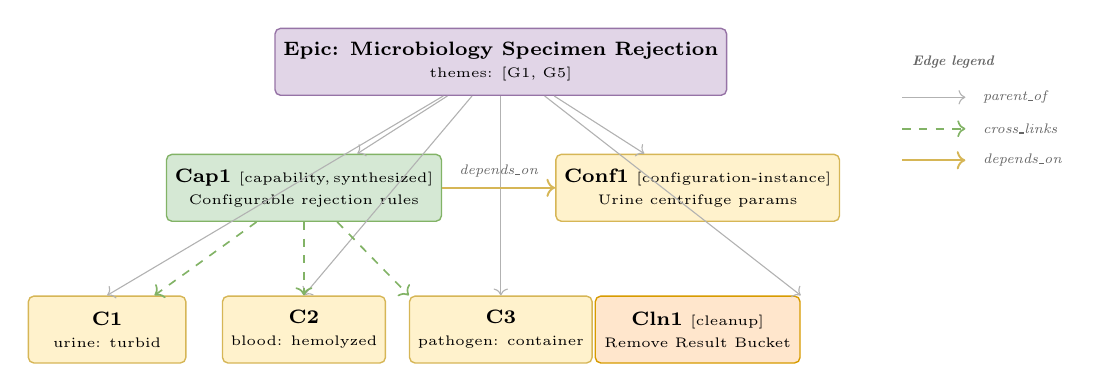
\begin{tikzpicture}[node distance=0.5cm]
  \node[ai, minimum width=3.4cm] (epic) at (5.5,4) {\textbf{Epic: Microbiology Specimen Rejection}\\\tiny themes: [G1, G5]};
  \node[dst, minimum width=2.6cm] (cap) at (3,2.4)
    {\textbf{Cap1} {\tiny [capability,\,synthesized]}\\\tiny Configurable rejection rules};
  \node[val, minimum width=2.6cm] (conf) at (8,2.4)
    {\textbf{Conf1} {\tiny [configuration-instance]}\\\tiny Urine centrifuge params};
  \node[val, minimum width=2.0cm] (c1) at (0.5,0.6) {\textbf{C1}\\\tiny urine: turbid};
  \node[val, minimum width=2.0cm] (c2) at (3,0.6)   {\textbf{C2}\\\tiny blood: hemolyzed};
  \node[val, minimum width=2.0cm] (c3) at (5.5,0.6) {\textbf{C3}\\\tiny pathogen: container};
  \node[xcut, minimum width=2.6cm] (cln) at (8,0.6) {\textbf{Cln1} {\tiny [cleanup]}\\\tiny Remove Result Bucket};
  \draw[->, draw=cmpdraw!50, line width=0.4pt] (epic) -- (cap);
  \draw[->, draw=cmpdraw!50, line width=0.4pt] (epic) -- (conf);
  \draw[->, draw=cmpdraw!50, line width=0.4pt] (epic) -- (c1.north);
  \draw[->, draw=cmpdraw!50, line width=0.4pt] (epic) -- (c2.north);
  \draw[->, draw=cmpdraw!50, line width=0.4pt] (epic) -- (c3.north);
  \draw[->, draw=cmpdraw!50, line width=0.4pt] (epic) -- (cln.north east);
  \draw[->, draw=outdraw, dashed, line width=0.6pt] (cap) -- (c1);
  \draw[->, draw=outdraw, dashed, line width=0.6pt] (cap) -- (c2);
  \draw[->, draw=outdraw, dashed, line width=0.6pt] (cap) -- (c3.north west);
  \draw[->, draw=valdraw, line width=0.7pt] (cap) -- node[lab,above]{depends\_on} (conf);
  \node[lab, anchor=west] at (10.6, 4.0)   {\textbf{Edge legend}};
  \draw[->, draw=cmpdraw!50, line width=0.4pt] (10.6,3.55) -- (11.4,3.55);
  \node[lab, anchor=west] at (11.5,3.55) {parent\_of};
  \draw[->, draw=outdraw, dashed, line width=0.6pt] (10.6,3.15) -- (11.4,3.15);
  \node[lab, anchor=west] at (11.5,3.15) {cross\_links};
  \draw[->, draw=valdraw, line width=0.7pt] (10.6,2.75) -- (11.4,2.75);
  \node[lab, anchor=west] at (11.5,2.75) {depends\_on};
\end{tikzpicture}
\end{figure}

\begin{tabularx}{\textwidth}{@{}>{\ttfamily}p{2.5cm}p{3.5cm}X@{}}
\toprule
\textbf{edge} & \textbf{direction} & \textbf{meaning} \\
\midrule
parent\_of & Epic $\rightarrow$ Story & Implicit Jira hierarchy (encoded in \texttt{epic\_id}). \\
cross\_links & Story $\leftrightarrow$ Story & Bidirectional association. Capability $\leftrightarrow$ concrete (synthesis); stage-split sibling sets. \\
depends\_on & Story $\rightarrow$ Story & Directed prerequisite. The Dependency Resolver topologically orders the backlog for sprint planning. \\
\bottomrule
\end{tabularx}

% =====================================================================
\section{Cross-SOP synthesis --- recurrence becomes capability}
% =====================================================================

\begin{figure}[H]
\centering
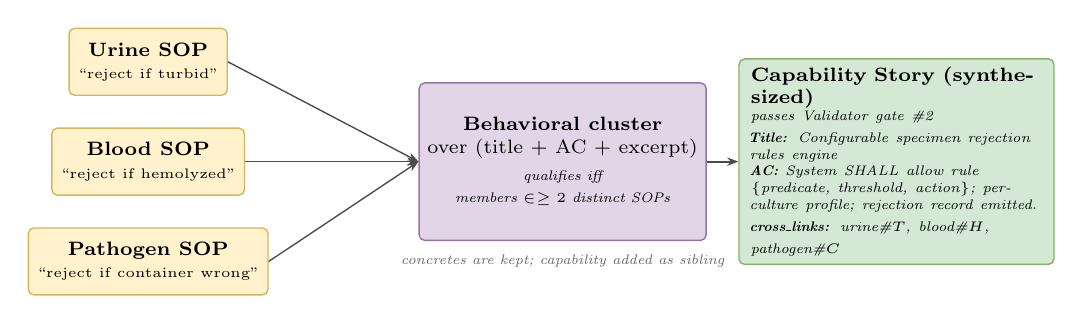
\begin{tikzpicture}[node distance=0.4cm]
  \node[val] (sop1) {\textbf{Urine SOP}\\\tiny ``reject if turbid''};
  \node[val, below=of sop1] (sop2) {\textbf{Blood SOP}\\\tiny ``reject if hemolyzed''};
  \node[val, below=of sop2] (sop3) {\textbf{Pathogen SOP}\\\tiny ``reject if container wrong''};
  \node[ai, right=2.2cm of sop2, minimum width=3.6cm, minimum height=2.0cm, align=center] (cluster)
    {\textbf{Behavioral cluster}\\\scriptsize over (title + AC + excerpt)\\[2pt]
     \tiny\itshape qualifies iff\\\tiny\itshape members $\in \geq 2$ distinct SOPs};
  \node[dst, right=of cluster, minimum width=4.0cm, minimum height=2.4cm, align=left, text width=3.7cm] (cap)
    {\textbf{Capability Story (synthesized)}\\\tiny\itshape passes Validator gate \#2\\[2pt]
     \tiny\textbf{Title:} Configurable specimen rejection rules engine\\
     \tiny\textbf{AC:} System SHALL allow rule \{predicate, threshold, action\}; per-culture profile; rejection record emitted.\\
     \tiny\textbf{cross\_links:} urine\#$T$, blood\#$H$, pathogen\#$C$};
  \draw[arr] (sop1.east) -- (cluster.west);
  \draw[arr] (sop2.east) -- (cluster.west);
  \draw[arr] (sop3.east) -- (cluster.west);
  \draw[arr, line width=0.7pt] (cluster.east) -- (cap.west);
  \node[lab, below=0.05cm of cluster] {concretes are kept; capability added as sibling};
\end{tikzpicture}
\end{figure}

The recurrence threshold ($\geq 2$ distinct SOPs) is tunable. With three SOPs in the POC, this means anything seen in two of three lifts. The synthesized capability story passes Validator gate \#2 before persistence.

% =====================================================================
\section{Cyto $\rightarrow$ Micro lineage (graph view)}
% =====================================================================

Three distinct mechanisms transfer information from Cyto to Micro. They operate at different times in the system's life cycle.

\begin{figure}[H]
\centering
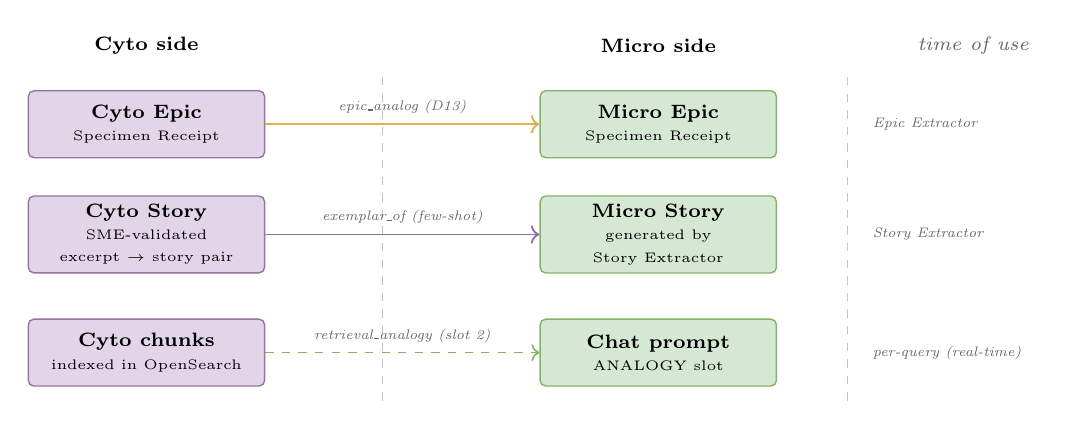
\begin{tikzpicture}[node distance=0.4cm]
  \node[font=\scriptsize\bfseries] at (1.5,4.6) {Cyto side};
  \node[font=\scriptsize\bfseries] at (8,4.6)   {Micro side};
  \node[font=\scriptsize\itshape, text=black!60] at (12.0,4.6) {time of use};
  \node[ai, minimum width=3.0cm] (cy_e) at (1.5,3.6)  {\textbf{Cyto Epic}\\\tiny Specimen Receipt};
  \node[dst, minimum width=3.0cm] (mi_e) at (8,3.6)   {\textbf{Micro Epic}\\\tiny Specimen Receipt};
  \draw[->, draw=valdraw, line width=0.7pt] (cy_e) -- node[lab,above]{epic\_analog (D13)} (mi_e);
  \node[lab, anchor=west] at (10.6,3.6) {Epic Extractor};
  \node[ai, minimum width=3.0cm] (cy_s) at (1.5,2.2)  {\textbf{Cyto Story}\\\tiny SME-validated\\\tiny excerpt $\rightarrow$ story pair};
  \node[dst, minimum width=3.0cm] (mi_s) at (8,2.2)   {\textbf{Micro Story}\\\tiny generated by\\\tiny Story Extractor};
  \draw[->, draw=aidraw, line width=0.7pt] (cy_s) -- node[lab,above]{exemplar\_of (few-shot)} (mi_s);
  \node[lab, anchor=west] at (10.6,2.2) {Story Extractor};
  \node[ai, minimum width=3.0cm] (cy_c) at (1.5,0.7)  {\textbf{Cyto chunks}\\\tiny indexed in OpenSearch};
  \node[dst, minimum width=3.0cm] (mi_p) at (8,0.7)   {\textbf{Chat prompt}\\\tiny ANALOGY slot};
  \draw[->, draw=outdraw, dashed, line width=0.6pt] (cy_c) -- node[lab,above]{retrieval\_analogy (slot 2)} (mi_p);
  \node[lab, anchor=west] at (10.6,0.7) {per-query (real-time)};
  \begin{scope}[on background layer]
    \draw[dashed, draw=cmpdraw!40] (4.5,4.2) -- (4.5,0.0);
    \draw[dashed, draw=cmpdraw!40] (10.4,4.2) -- (10.4,0.0);
  \end{scope}
\end{tikzpicture}
\end{figure}

\begin{tabularx}{\textwidth}{@{}>{\ttfamily}p{3.0cm}p{4.0cm}X@{}}
\toprule
\textbf{mechanism} & \textbf{direction} & \textbf{when it fires / what flows} \\
\midrule
epic\_analog & Cyto Epic $\rightarrow$ Micro Epic & At Epic-Extractor time. Just an ID reference --- recorded for SME traceability (D13). \\
exemplar\_of & Cyto Story $\rightarrow$ Micro Story & At Story-Extractor time. The Cyto (excerpt $\rightarrow$ Story) pair lands in the prompt as an in-context example. \\
retrieval\_analogy & Cyto chunks $\rightarrow$ chat prompt & Per-query, real-time. Retrieved Cyto excerpts populate the ANALOGY context section. \emph{Adapt, don't copy.} \\
\bottomrule
\end{tabularx}

The same Cyto material thus serves three roles: a curated few-shot teaching set, an indexed corpus for live retrieval, and a structural reference at the Epic level.

% =====================================================================
\section{v3.2 ANALOGY map (graph view) --- explicit cross-discipline links}
% =====================================================================

When a discipline's theme catalog diverges from its parent (Histology drops G7, adds H1--H4), the ANALOGY map records the cross-catalog correspondences explicitly. Each link is typed --- the legend shows what each line style means.

\begin{figure}[H]
\centering
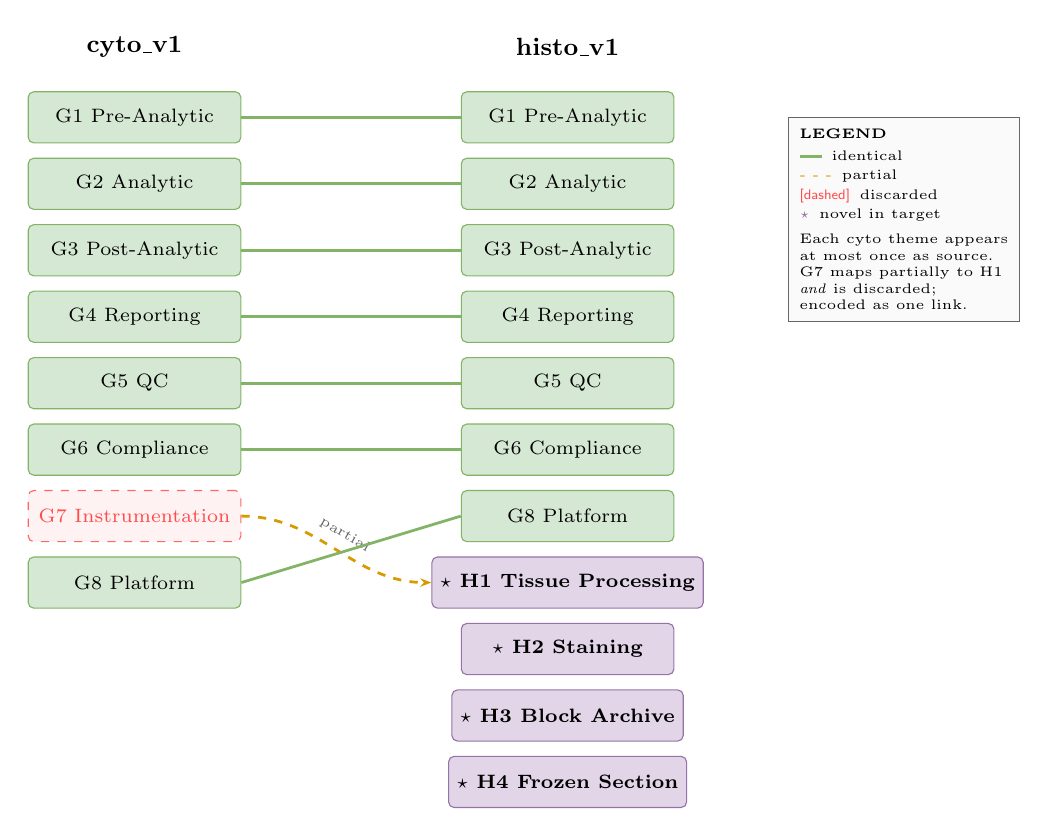
\begin{tikzpicture}[node distance=0.18cm and 1.8cm,
    tnode/.style={rectangle, rounded corners=2pt, draw=outdraw, fill=outfill, line width=0.4pt, align=center, font=\scriptsize, inner sep=3pt, minimum width=2.7cm, minimum height=0.65cm},
    tdiscard/.style={tnode, draw=red!60, fill=red!5, dashed, text=red!70},
    tnovel/.style={tnode, draw=aidraw, fill=aifill, font=\scriptsize\bfseries}]

  \node[font=\bfseries\small] (chc) at (0,0) {cyto\_v1};
  \node[font=\bfseries\small] (hhd) at (5.5,0) {histo\_v1};

  \node[tnode, below=0.3cm of chc] (cg1) {G1 Pre-Analytic};
  \node[tnode, below=of cg1] (cg2) {G2 Analytic};
  \node[tnode, below=of cg2] (cg3) {G3 Post-Analytic};
  \node[tnode, below=of cg3] (cg4) {G4 Reporting};
  \node[tnode, below=of cg4] (cg5) {G5 QC};
  \node[tnode, below=of cg5] (cg6) {G6 Compliance};
  \node[tdiscard, below=of cg6] (cg7) {G7 Instrumentation};
  \node[tnode, below=of cg7] (cg8) {G8 Platform};

  \node[tnode] (hg1) at (5.5, |-cg1) {G1 Pre-Analytic};
  \node[tnode, below=of hg1] (hg2) {G2 Analytic};
  \node[tnode, below=of hg2] (hg3) {G3 Post-Analytic};
  \node[tnode, below=of hg3] (hg4) {G4 Reporting};
  \node[tnode, below=of hg4] (hg5) {G5 QC};
  \node[tnode, below=of hg5] (hg6) {G6 Compliance};
  \node[tnode, below=of hg6] (hg8) {G8 Platform};
  \node[tnovel, below=of hg8] (hh1) {$\star$ H1 Tissue Processing};
  \node[tnovel, below=of hh1] (hh2) {$\star$ H2 Staining};
  \node[tnovel, below=of hh2] (hh3) {$\star$ H3 Block Archive};
  \node[tnovel, below=of hh3] (hh4) {$\star$ H4 Frozen Section};

  \draw[outdraw, line width=1pt] (cg1.east) -- (hg1.west);
  \draw[outdraw, line width=1pt] (cg2.east) -- (hg2.west);
  \draw[outdraw, line width=1pt] (cg3.east) -- (hg3.west);
  \draw[outdraw, line width=1pt] (cg4.east) -- (hg4.west);
  \draw[outdraw, line width=1pt] (cg5.east) -- (hg5.west);
  \draw[outdraw, line width=1pt] (cg6.east) -- (hg6.west);
  \draw[xdraw, line width=1pt, dashed, ->, >={Stealth[length=4pt]}] (cg7.east) to[out=0,in=180] node[lab, sloped, above, font=\tiny]{partial} (hh1.west);
  \draw[outdraw, line width=1pt] (cg8.east) -- (hg8.west);

  % legend
  \node[anchor=north west, font=\tiny, align=left, draw=cmpdraw, fill=notefill, line width=0.3pt, inner sep=4pt] (leg) at (8.3, |-cg1) {%
    \textbf{LEGEND}\\[2pt]
    {\color{outdraw}\rule[0.4ex]{1.2em}{1.0pt}}\, identical\\[1pt]
    {\color{xdraw}- - -}\, partial\\[1pt]
    {\color{red!70}\sffamily\textsf{[dashed]}}\, discarded\\[1pt]
    {\color{aidraw}$\star$}\, novel in target\\[3pt]
    Each cyto theme appears\\ at most once as source.\\ G7 maps partially to H1\\ \emph{and} is discarded;\\ encoded as one link.};
\end{tikzpicture}
\caption{ANALOGY map (cyto\_v1 $\leftrightarrow$ histo\_v1). 6 identical theme links, 1 partial (G7$\rightarrow$H1), 4 novel-in-target (H1--H4). H1 has no separate \texttt{novel\_in\_target} edge because the partial G7$\rightarrow$H1 link already records its origin.}
\end{figure}

The ANALOGY map drives the ANALOGY retrieval slot for cross-discipline queries: when a Histo question wants Cyto context, the map filters Cyto chunks down to themes that have a target-side correspondent.

% =====================================================================
\section{Ingestion substrate --- S3 to indexed chunks}
% =====================================================================

\begin{figure}[H]
\centering
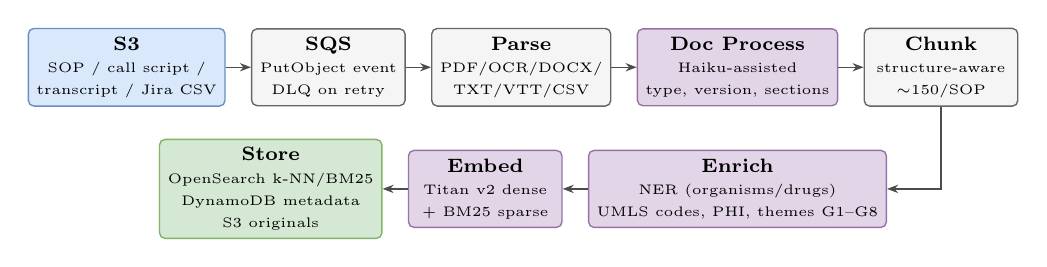
\begin{tikzpicture}[node distance=0.32cm]
  \node[src] (s3in) {\textbf{S3}\\\tiny SOP / call script /\\\tiny transcript / Jira CSV};
  \node[cmp, right=of s3in] (sqs) {\textbf{SQS}\\\tiny PutObject event\\\tiny DLQ on retry};
  \node[cmp, right=of sqs] (parse) {\textbf{Parse}\\\tiny PDF/OCR/DOCX/\\\tiny TXT/VTT/CSV};
  \node[ai, right=of parse] (doc) {\textbf{Doc Process}\\\tiny Haiku-assisted\\\tiny type, version, sections};
  \node[cmp, right=of doc] (chunk) {\textbf{Chunk}\\\tiny structure-aware\\\tiny $\sim$150/SOP};
  \node[ai, below=0.55cm of doc] (enrich) {\textbf{Enrich}\\\tiny NER (organisms/drugs)\\\tiny UMLS codes, PHI, themes G1--G8};
  \node[ai, left=of enrich] (embed) {\textbf{Embed}\\\tiny Titan v2 dense\\\tiny + BM25 sparse};
  \node[dst, left=of embed] (store) {\textbf{Store}\\\tiny OpenSearch k-NN/BM25\\\tiny DynamoDB metadata\\\tiny S3 originals};
  \draw[arr] (s3in) -- (sqs);
  \draw[arr] (sqs) -- (parse);
  \draw[arr] (parse) -- (doc);
  \draw[arr] (doc) -- (chunk);
  \draw[arr] (chunk.south) |- (enrich.east);
  \draw[arr] (enrich) -- (embed);
  \draw[arr] (embed) -- (store);
\end{tikzpicture}
\end{figure}

\textbf{I/O trace --- one document through the pipeline} (\texttt{SOP-MICRO-014\_Gram-Stain\_v3.docx}):

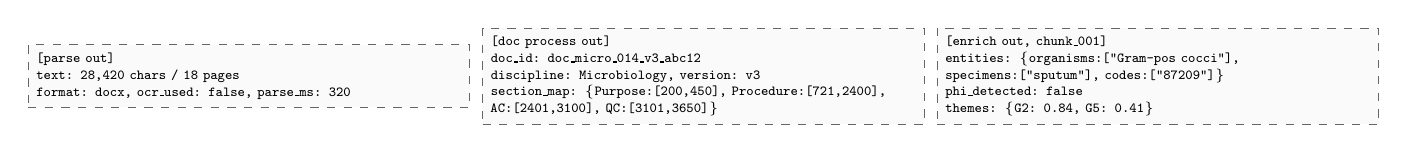
\begin{tikzpicture}[node distance=0.15cm]
  \node[io, text width=5.4cm] (i1) {\textbf{[parse out]}\\
text: 28{,}420 chars / 18 pages\\
format: docx, ocr\_used: false, parse\_ms: 320};
  \node[io, right=of i1, text width=5.4cm] (i2) {\textbf{[doc process out]}\\
doc\_id: doc\_micro\_014\_v3\_abc12\\
discipline: Microbiology, version: v3\\
section\_map: \{Purpose:[200,450], Procedure:[721,2400], AC:[2401,3100], QC:[3101,3650]\}};
  \node[io, right=of i2, text width=5.4cm] (i3) {\textbf{[enrich out, chunk\_001]}\\
entities: \{organisms:["Gram-pos cocci"], specimens:["sputum"], codes:["87209"]\}\\
phi\_detected: false\\
themes: \{G2: 0.84, G5: 0.41\}};
\end{tikzpicture}

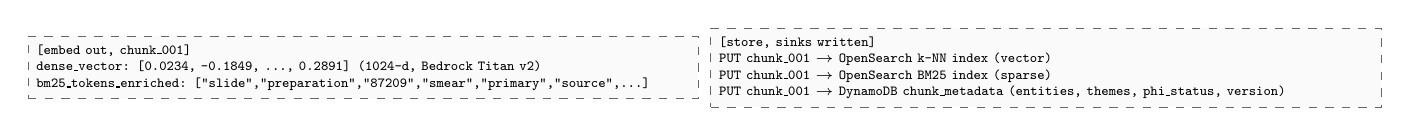
\begin{tikzpicture}[node distance=0.15cm]
  \node[io, text width=8.3cm] (i4) {\textbf{[embed out, chunk\_001]}\\
dense\_vector: [0.0234, -0.1849, ..., 0.2891]\, (1024-d, Bedrock Titan v2)\\
bm25\_tokens\_enriched: ["slide","preparation","87209","smear","primary","source",...]};
  \node[io, right=of i4, text width=8.3cm] (i5) {\textbf{[store, sinks written]}\\
PUT chunk\_001 $\rightarrow$ OpenSearch k-NN index (vector)\\
PUT chunk\_001 $\rightarrow$ OpenSearch BM25 index (sparse)\\
PUT chunk\_001 $\rightarrow$ DynamoDB \texttt{chunk\_metadata} (entities, themes, phi\_status, version)};
\end{tikzpicture}

% =====================================================================
\section{Retrieval substrate --- per query, real-time}
% =====================================================================

\begin{figure}[H]
\centering
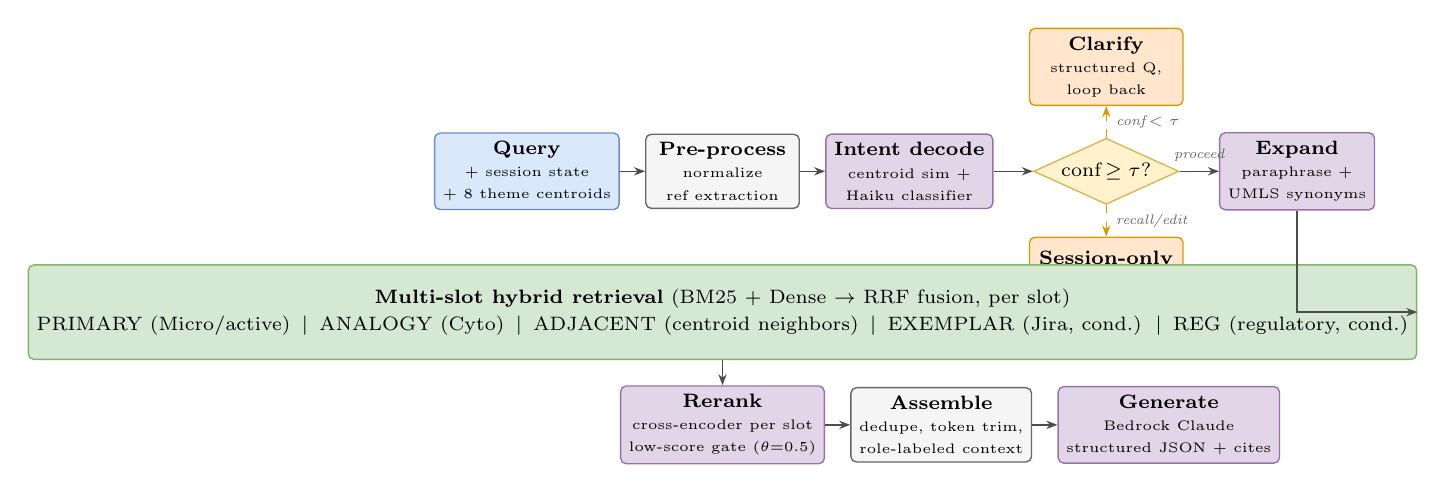
\begin{tikzpicture}[node distance=0.32cm]
  \node[src] (q) {\textbf{Query}\\\tiny + session state\\\tiny + 8 theme centroids};
  \node[cmp, right=of q] (pre) {\textbf{Pre-process}\\\tiny normalize\\\tiny ref extraction};
  \node[ai, right=of pre] (intent) {\textbf{Intent decode}\\\tiny centroid sim +\\\tiny Haiku classifier};
  \node[decision, right=0.5cm of intent] (dec) {\scriptsize conf\,$\geq\tau$?};
  \node[ai, right=0.5cm of dec] (exp) {\textbf{Expand}\\\tiny paraphrase +\\\tiny UMLS synonyms};
  \node[xcut, above=0.4cm of dec] (clar) {\textbf{Clarify}\\\tiny structured Q,\\\tiny loop back};
  \node[xcut, below=0.4cm of dec] (sess) {\textbf{Session-only}\\\tiny recall / edit};
  \node[dst, below=0.7cm of pre, minimum width=10.5cm, minimum height=1.2cm, align=center] (slots)
    {\textbf{Multi-slot hybrid retrieval} (BM25 + Dense $\rightarrow$ RRF fusion, per slot)\\[2pt]
     \scriptsize PRIMARY (Micro/active) \,$|$\, ANALOGY (Cyto) \,$|$\, ADJACENT (centroid neighbors) \,$|$\, EXEMPLAR (Jira, cond.) \,$|$\, REG (regulatory, cond.)};
  \node[ai, below=0.32cm of slots] (rer) {\textbf{Rerank}\\\tiny cross-encoder per slot\\\tiny low-score gate ($\theta$=0.5)};
  \node[cmp, right=of rer] (asm) {\textbf{Assemble}\\\tiny dedupe, token trim,\\\tiny role-labeled context};
  \node[ai, right=of asm] (gen) {\textbf{Generate}\\\tiny Bedrock Claude\\\tiny structured JSON + cites};
  \draw[arr] (q) -- (pre);
  \draw[arr] (pre) -- (intent);
  \draw[arr] (intent) -- (dec);
  \draw[arr] (dec) -- node[lab, above]{proceed} (exp);
  \draw[arrdash] (dec) -- node[lab, right]{conf\,$<\tau$} (clar);
  \draw[arrdash] (dec) -- node[lab, right]{recall/edit} (sess);
  \draw[arr] (exp.south) |- (slots.east);
  \draw[arr] (slots) -- (rer);
  \draw[arr] (rer) -- (asm);
  \draw[arr] (asm) -- (gen);
\end{tikzpicture}
\end{figure}

\textbf{I/O trace --- one query: ``Generate epics for specimen rejection in microbiology''}

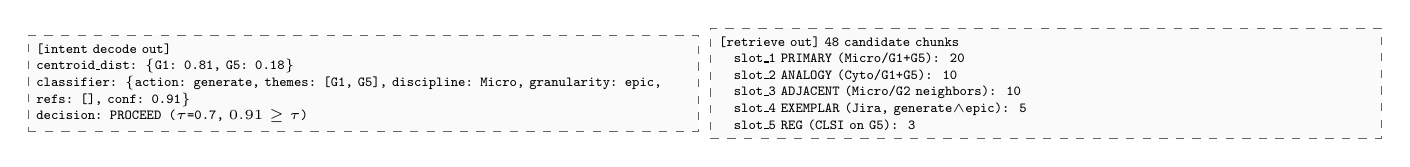
\begin{tikzpicture}[node distance=0.15cm]
  \node[io, text width=8.3cm] (q1) {\textbf{[intent decode out]}\\
centroid\_dist: \{G1: 0.81, G5: 0.18\}\\
classifier: \{action: generate, themes: [G1, G5], discipline: Micro, granularity: epic, refs: [], conf: 0.91\}\\
decision: PROCEED\, ($\tau$=0.7, $0.91 \geq \tau$)};
  \node[io, right=of q1, text width=8.3cm] (q2) {\textbf{[retrieve out]} 48 candidate chunks\\
\quad slot\_1 PRIMARY (Micro/G1+G5):\, 20\\
\quad slot\_2 ANALOGY (Cyto/G1+G5):\, 10\\
\quad slot\_3 ADJACENT (Micro/G2 neighbors):\, 10\\
\quad slot\_4 EXEMPLAR (Jira, generate$\wedge$epic):\, 5\\
\quad slot\_5 REG (CLSI on G5):\, 3};
\end{tikzpicture}

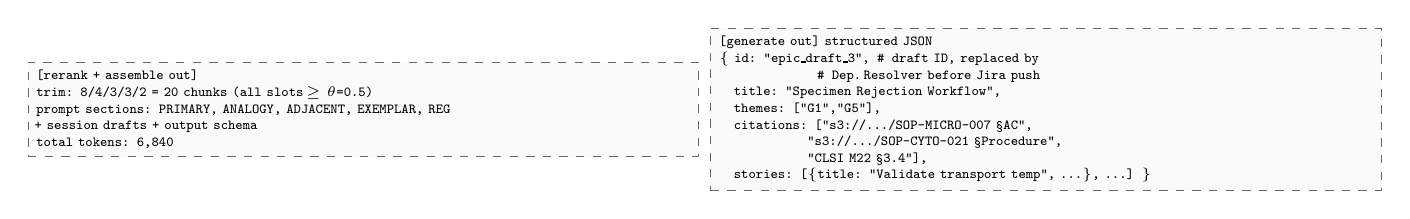
\begin{tikzpicture}[node distance=0.15cm]
  \node[io, text width=8.3cm] (q3) {\textbf{[rerank + assemble out]}\\
trim: 8/4/3/3/2 = 20 chunks (all slots\,$\geq\theta$=0.5)\\
prompt sections: PRIMARY, ANALOGY, ADJACENT, EXEMPLAR, REG\\
+ session drafts + output schema\\
total tokens: 6{,}840};
  \node[io, right=of q3, text width=8.3cm] (q4) {\textbf{[generate out]} structured JSON\\
\{ id: "epic\_draft\_3",\,\,\,\#\, draft ID, replaced by\\
\quad\,\,\,\,\,\,\,\,\,\,\,\,\,\,\,\,\,\,\,\,\,\,\,\,\,\,\,\,\,\,\,\,\,\,\#\, Dep.\,Resolver before Jira push\\
\quad title: "Specimen Rejection Workflow",\\
\quad themes: ["G1","G5"],\\
\quad citations: ["s3://.../SOP-MICRO-007 \S AC",\\
\quad\quad\quad\quad\quad\quad "s3://.../SOP-CYTO-021 \S Procedure",\\
\quad\quad\quad\quad\quad\quad "CLSI M22 \S 3.4"],\\
\quad stories: [\{title: "Validate transport temp", ...\}, ...] \}};
\end{tikzpicture}

% =====================================================================
\section{Validator --- shape-aware revise/escalate flow}
% =====================================================================

\begin{figure}[H]
\centering
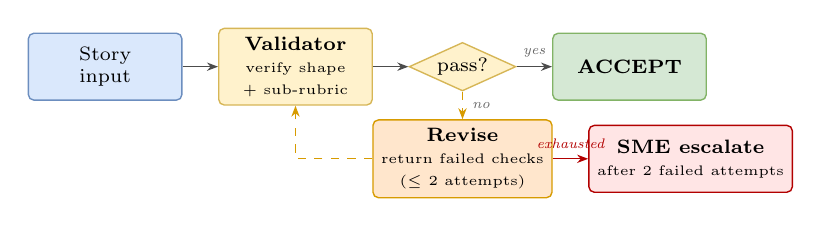
\begin{tikzpicture}[node distance=0.45cm]
  \node[src] (in) {Story\\input};
  \node[val, right=of in] (v) {\textbf{Validator}\\\tiny verify shape\\\tiny + sub-rubric};
  \node[decision, right=of v] (p) {\scriptsize pass?};
  \node[dst, right=of p] (acc) {\textbf{ACCEPT}};
  \node[xcut, below=0.35cm of p] (rev) {\textbf{Revise}\\\tiny return failed checks\\\tiny ($\leq$ 2 attempts)};
  \node[blk, draw=red!70!black, fill=red!10, right=of rev] (esc) {\textbf{SME escalate}\\\tiny after 2 failed attempts};
  \draw[arr] (in) -- (v);
  \draw[arr] (v) -- (p);
  \draw[arr] (p) -- node[lab, above]{yes} (acc);
  \draw[arrdash] (p) -- node[lab, right]{no} (rev);
  \draw[arrdash] (rev) -| (v);
  \draw[arr, draw=red!70!black] (rev) -- node[lab, above, text=red!70!black]{exhausted} (esc);
\end{tikzpicture}
\end{figure}

\textbf{Sub-rubrics by shape (cheat sheet):}
\begin{itemize}
  \item \textbf{Capability:} MUST/SHALL on every AC; testable; no ambiguous quantifiers (``appropriate'', ``relevant'', ``necessary''); configurability boundaries called out; SOP citation present and resolves; complexity S/M/L; edge cases enumerated.
  \item \textbf{Stage-split:} stage explicit in title; entry/exit observable per stage; siblings enumerated and cross-linked; transition contract clear; boundary cases handled.
  \item \textbf{Configuration-instance:} typed concrete values (units / enums / nullable rules); target table or profile named (e.g.\ \texttt{cultures/urine.yaml\#centrifugation}); SOP excerpt cited verbatim; scope (culture/lab) stated. \emph{MUST/SHALL not required.}
  \item \textbf{Cleanup:} target artifact named (id, screen path, file path); before/after observable; regression risk acknowledged; DoD includes a smoke test or QA path. \emph{MUST/SHALL not required.}
\end{itemize}

% =====================================================================
\section{What ships --- Output A (Jira) and Output B (YAML)}
% =====================================================================

\textbf{Output A --- Jira artifacts.} The connected Epic / Story DAG (graph above), pushed to Jira via REST. The graph is what the dev team works against; the YAML profile (Output B) is what their code consumes at runtime.

\textbf{Output B --- Per-culture YAML configuration profile.} One YAML file per culture in scope. Carries the concrete typed values that \texttt{configuration-instance} Stories' AC referenced. Profiles are versioned, dated, and cite back to the SOPs they draw from. \textbf{The Story body never duplicates these values} --- it references them by \texttt{related\_story\_ac}, so a single source of truth is preserved.

The profile is partitioned by workflow stage so an engineer can find the right block at a glance:
\begin{itemize}
  \item \texttt{pre\_analytic} --- before the specimen reaches the bench: collection, transport, rejection predicates.
  \item \texttt{analytic} --- the bench work itself: centrifugation, inoculation, incubation.
  \item \texttt{post\_analytic} --- after the result: reporting thresholds, downstream notifications.
\end{itemize}

\subsection{Full profile structure (\texttt{cultures/urine.yaml})}

\noindent\texttt{\scriptsize profile:\\
\hspace*{1em}culture: urine\,\,\,\,\,\,\,\,\,\,\,\,\,\,\,\,\,\,\,\,\,\,\,\,\,\,\,\,\,\,\,\,\#\, urine $|$ blood $|$ target\_pathogen\\
\hspace*{1em}version: 3\\
\hspace*{1em}effective\_date: 2026-04-15\\
\hspace*{1em}source\_sops: [doc\_micro\_014\_v3, doc\_micro\_022\_v1]\\
\\
pre\_analytic:\\
\hspace*{1em}collection:\\
\hspace*{2em}container:\,\,\,\,\,\,\{value: "sterile cup", units: enum, citation: "doc\_micro\_014\_v3 \S 1.2 L8"\}\\
\hspace*{2em}volume\_min:\,\,\,\,\{value: 10, units: mL, citation: "doc\_micro\_014\_v3 \S 1.2 L11"\}\\
\hspace*{1em}transport:\\
\hspace*{2em}temp\_range:\,\,\,\,\{min: 2, max: 8, units: degC, citation: "doc\_micro\_014\_v3 \S 1.4 L18-19"\}\\
\hspace*{2em}time\_max:\,\,\,\,\,\,\{value: 4, units: h, citation: "doc\_micro\_014\_v3 \S 1.4 L20"\}\\
\hspace*{1em}rejection\_predicates:\\
\hspace*{2em}- id: REJ\_TURBID\\
\hspace*{3em}condition: "turbidity > threshold"\\
\hspace*{3em}threshold: \{value: 200, units: NTU\}\\
\hspace*{3em}action: reject\\
\hspace*{3em}citation: "doc\_micro\_014\_v3 \S 1.5 L24"\\
\\
analytic:\\
\hspace*{1em}centrifugation:\\
\hspace*{2em}speed:\,\,\,\,\,\{value: 1500, units: g,\,\,\,\,citation: "doc\_micro\_014\_v3 \S 3.2 L41-43"\}\\
\hspace*{2em}duration: \{value: 5,\,\,\,\,units: min,\,\,\,citation: "doc\_micro\_014\_v3 \S 3.2 L44"\}\\
\hspace*{2em}temp:\,\,\,\,\,\,\{value: 4,\,\,\,\,units: degC,\,\,citation: "doc\_micro\_014\_v3 \S 3.2 L45"\}\\
\hspace*{1em}inoculation:\\
\hspace*{2em}media:\\
\hspace*{3em}- \{type: BAP, volume\_uL: 10, citation: "doc\_micro\_014\_v3 \S 4.1 L52"\}\\
\hspace*{3em}- \{type: MAC, volume\_uL: 10, citation: "doc\_micro\_014\_v3 \S 4.1 L53"\}\\
\hspace*{2em}incubation: \{temp: 35, atmosphere: "5\% CO2", duration\_h: 18,\\
\hspace*{4em}citation: "doc\_micro\_014\_v3 \S 4.3 L60"\}\\
\\
post\_analytic:\\
\hspace*{1em}reporting:\\
\hspace*{2em}cfu\_threshold: \{value: 100000, units: CFU\_per\_mL,\\
\hspace*{4em}citation: "doc\_micro\_014\_v3 \S 6.1 L88"\}\\
\\
related\_story\_acs:\,\,\,\,\,\,\,\#\, back-references to Stories that consume this profile\\
\hspace*{1em}- STORY-MICRO-1042\#AC-2\,\,\,\#\, Configurable rejection rules engine\\
\hspace*{1em}- STORY-MICRO-1077\#AC-1\,\,\,\#\, Centrifugation step}

\subsection{How a Story's AC references the profile}

A \texttt{configuration-instance} Story's AC carries the citation; the profile is what gets read by code. Example --- \texttt{STORY-MICRO-1077}:

\noindent\texttt{\scriptsize acceptance\_criteria:\\
\hspace*{1em}- when: "urine profile loaded"\\
\hspace*{2em}then: "centrifuge step uses cultures/urine.yaml\#analytic.centrifugation"\\
\hspace*{2em}expected\_value: "speed=1500g, duration=5min, temp=4degC"}

\subsection{Where to put a value: Story body vs.\ profile}

\begin{tabularx}{\textwidth}{@{}p{6.5cm}X@{}}
\toprule
\textbf{If the value is\ldots} & \textbf{Put it in\ldots} \\
\midrule
The same across cultures and parameterizable in the rules engine & Story body as parameter spec (capability shape) \\
Different per culture / per lab & YAML profile (configuration-instance shape) \\
A literal constant in the rejection logic & Profile, with the Story's AC pointing at it \\
\bottomrule
\end{tabularx}

% =====================================================================
\section{Cross-cutting}
% =====================================================================

KMS encryption at rest and in transit; IAM least-privilege with VPC endpoints (Bedrock calls stay in-VPC); DLQ for parse / OCR / embed failures; CloudWatch metrics and alarms (e.g.\ OCR fail-rate $> 5\%$); CloudTrail audit log on every API call; idempotent ingestion via content-hash dedupe.

\textbf{Generalization (v3.2):} when Histology arrives, Theme Discovery runs once as pre-flight to warm-start \texttt{histo\_v1} from \texttt{cyto\_v1} (most themes inherited; novel ones SME-ratified). The main pipeline then runs unchanged in shape, with the Epic Extractor in conditioned mode bootstrapping \texttt{histo\_epic\_v1} from \texttt{cyto\_epic\_v1}. No model retraining at any stage.

\end{document}
